\chapter{Renderer: Architecture and Implementation}
\label{ch:architecture}

This chapter describes the renderer itself: a from-scratch CUDA/OptiX volumetric path tracer for the
Gaussian kernel-mixture volumes of \Cref{sec:kernel-mixture}. Its design answers one question
differently from the reference: \emph{given a camera ray, how is the next scattering event found?}
The reference~\cite{DSYG} marches the ray segment by segment, advancing from one primitive
boundary to the next by a running minimum. Where primitives overlap, it root-finds the scatter
distance numerically; single-primitive segments it inverts in closed form. This renderer instead
collects all of a ray's primitives in a \emph{single} acceleration-structure traversal. It then
samples the scatter distance in \emph{closed form even across overlaps}, with no sorting, no
marching, and no root-finding. The two halves of that design---single-trace collection
(\Cref{sec:collection}) and analog-decomposition scatter sampling (\Cref{sec:adt})---are the
thesis's primary contribution. The supporting components (direct lighting, data structures, and the
OptiX configuration) are described in \Crefrange{sec:direct-lighting}{sec:gpu-impl}.

\section{Pipeline overview}
\label{sec:pipeline}

The renderer ingests a set of Gaussian primitives: a PLY file of centres, covariances encoded as
scale + rotation quaternion, densities ($\sigma_t$ amplitudes), and albedos (the
scattered fraction $\sigma_s/\sigma_t$, \Cref{sec:volumetric-light-transport}). It
builds a two-level OptiX acceleration
structure over them (\Cref{sec:gpu-impl}) and path-traces the image in a single
\emph{megakernel}---one GPU kernel containing the entire per-pixel path-tracing loop
(\Cref{sec:gpu-impl})---launched
per pixel. Each path repeats four steps per bounce. It \emph{collects} the primitives the current
ray segment intersects (one trace), then \emph{samples} a scattering distance from them (the argmin
of per-primitive free flights). It \emph{shades} the event (computes its direct lighting) by next-event estimation
against the environment, and \emph{continues} along a phase-sampled direction until Russian roulette terminates
the path. Per-pixel
radiance is accumulated across samples by a single-pass online mean (\Cref{sec:direct-lighting}). The
entire bounce loop lives inside the ray-generation program; \Cref{sec:gpu-impl} explains why this
megakernel structure, rather than a wavefront of separate kernels, is the right fit for this
workload. \Cref{fig:pipeline} contrasts the per-bounce work of the reference with this renderer's.

\begin{figure}[htp]
  \centering
  \resizebox{\linewidth}{!}{%
  \begin{tikzpicture}[
      font=\small,
      box/.style={draw, rounded corners, minimum height=9mm, text width=20mm,
                  align=center, inner sep=3pt},
      gone/.style={box, dashed, text=black!55},
      >=Stealth, node distance=6mm and 7mm,
    ]
    % Reference pipeline
    \node[box]               (r1) {Trace + march\\ ($\times H$)};
    \node[gone, right=of r1] (r2) {Select next\\ boundary};
    \node[gone, right=of r2] (r3) {Bisection /\\ Newton};
    \node[box,  right=of r3] (r4) {Scatter\\ at $t$};
    \draw[->] (r1)--(r2); \draw[->] (r2)--(r3); \draw[->] (r3)--(r4);
    \node[anchor=east] at ([xshift=-4mm]r1.west) {\textbf{Reference}};
    \node[font=\scriptsize\itshape, text=black!55, above=1.5mm of r2, xshift=13.5mm]
         {eliminated by the argmin sampler};
    % This renderer's pipeline
    \node[box, below=14mm of r1] (o1) {Single any-hit\\ trace};
    \node[box, right=of o1]      (o2) {Keep entries,\\ exits analytic};
    \node[box, right=of o2]      (o3) {Argmin of\\ free flights};
    \node[box, right=of o3]      (o4) {Scatter\\ at $t$};
    \draw[->] (o1)--(o2); \draw[->] (o2)--(o3); \draw[->] (o3)--(o4);
    \node[font=\scriptsize, below=0.5mm of o3] {$O(A{+}H)$, unordered};
    \node[anchor=east] at ([xshift=-4mm]o1.west) {\textbf{This renderer}};
  \end{tikzpicture}%
  }
  \caption{Per-bounce scatter sampling, reference versus this renderer. The reference marches the ray
  boundary by boundary---one traversal per step, maintaining the overlapping-primitive set and
  selecting the next boundary by a running minimum---and root-finds the scatter distance within each
  segment. This renderer gathers all entries in a single any-hit traversal and takes the argmin of
  closed-form per-primitive free flights (the matching exits computed analytically rather than traced),
  eliminating the per-segment boundary selection and the root-find (dashed) entirely. ($H$:
the number of primitives the ray crosses; $A$: the number containing its origin;
\Cref{sec:collection}.)}
  \label{fig:pipeline}
\end{figure}

\section{Single-trace primitive collection}
\label{sec:collection}

To sample a scattering event along a ray, the renderer must know which primitives the ray passes
through and over what intervals. The reference constructs this information incrementally, advancing the
ray from one primitive boundary to the next and issuing a fresh acceleration-structure query at each
step. For a ray crossing $H$ overlapping primitives this is $O(H)$ traversals. This renderer's
collection scheme rests on the observation that every primitive is a bounded convex
region (its $3\sigma$ support ellipsoid, \Cref{sec:kernel-mixture}---a
transformed unit sphere, \Cref{sec:gpu-impl}). \emph{All} of the ray's entry points can therefore be
gathered in a \emph{single} traversal, and the corresponding exits then computed analytically.

Concretely, the scene is traced once per scattering event with an \emph{any-hit} program and no
closest-hit program (the ray flag \texttt{OPTIX\_\allowbreak RAY\_\allowbreak FLAG\_\allowbreak DISABLE\_\allowbreak CLOSESTHIT}). Because any-hit
fires for every intersection without terminating the ray, a single trace visits every primitive the
ray meets. OptiX's built-in sphere intersector natively provides one entry hit per primitive (a contract
revisited in \Cref{ch:optimization}). The any-hit program therefore records only \emph{entries}:
each a pair of hit distance $t_{\text{hit}}$ and primitive index, appended to a
per-ray buffer. (Back-face culling---discarding intersections with geometry facing away from the ray,
here the shell's interior, exit-side faces---\texttt{OPTIX\_\allowbreak RAY\_\allowbreak FLAG\_\allowbreak CULL\_\allowbreak BACK\_\allowbreak FACING\_\allowbreak TRIANGLES}, serves the same role only for the tessellated-icosphere variant of \Cref{ch:optimization}.) The matching exit of
any primitive is not traced at all: since the primitive's geometry is known, the exit distance follows
in closed form from the ray--sphere intersection. One traversal therefore replaces the reference's
$H$ (one per crossed boundary), and the buffer holds exactly the data the scatter sampler needs.

The entry buffer is a structure-of-arrays, \texttt{HitBufferSoA}, storing the hit distances and
primitive indices in separate arrays (\num{4} bytes and \num{2} bytes per entry respectively). The
sampler's sequential scan over distances therefore touches only the \num{4}-byte distance array,
halving its cache footprint. It is a per-ray buffer held in fast local memory
with a fixed capacity (\Cref{sec:gpu-impl}). Overflow is \emph{detected} rather than corrected: a
dropped hit biases the pixel toward under-absorption, but a device counter flags the event instead of
letting it pass silently. Two categories of primitive contribute to a scattering event. The first is
the primitives the ray is already \emph{inside} at the segment's start, tracked in an \emph{active
set}. (The camera may begin inside the medium; after a scatter, the new ray starts inside whatever
primitives contain the scatter point.) The second is the primitives the ray \emph{enters} along the
segment, delivered by the trace into the
hit buffer. The sampler in \Cref{sec:adt} draws candidates from both.

\section{Analytic optical depth}
\label{sec:analytic-od}

The property that makes both single-trace collection and closed-form scatter sampling possible is the
analytic optical depth of a single Gaussian (\Cref{sec:kernel-mixture}). The whitened-space derivation
below follows the reference~\cite{DSYG}, recast in the notation used throughout. Primitive $k$'s
extinction is
\[
  \sigma_{t,k}(\bm{x}) = C_k\,\exp\!\big(-\tfrac12\lVert S_k^{-1}R_k^{\!\top}(\bm{x}-\bm{\mu}_k)\rVert^2\big),
\]
with rotation $R_k$, per-axis scales $s_{ki}$ (the Gaussian's standard deviation along principal axis
$i\in\{1,2,3\}$) collected in $S_k=\operatorname{diag}(s_{ki})$, and peak extinction $C_k=\bar\sigma_{t,k}\big((2\pi)^{3/2}\prod_i s_{ki}\big)^{-1}$,
where $\bar\sigma_{t,k}$ is the primitive's stored extinction mass (the mass-normalised
convention of \Cref{sec:kernel-mixture}); $\sigma_{t,k}(\cdot)$ with an argument always
denotes the field, bare $\bar\sigma_{t,k}$ the scalar parameter. Substituting the ray
$\bm{r}(t)=\bm{o}+t\bm{\omega}$ and \emph{whitening} carries the exponent to a one-dimensional
quadratic (\Cref{fig:optical-depth}):
\[
  \bm{y}(t)=S_k^{-1}R_k^{\!\top}\big(\bm{r}(t)-\bm{\mu}_k\big)=\bm{a}+t\bm{b},
  \qquad
  \bm{a}=S_k^{-1}R_k^{\!\top}(\bm{o}-\bm{\mu}_k),
  \qquad
  \bm{b}=S_k^{-1}R_k^{\!\top}\bm{\omega}.
\]
Whitening is the affine change of coordinates that carries primitive
$k$'s anisotropic Gaussian to the \emph{standard} isotropic Gaussian (unit variance, centred at the
origin). It is a bijection because $R_k$ is orthogonal and $S_k$ diagonal with positive entries. The
ray therefore stays a straight line $\bm{a}+s\bm{b}$, and the extinction along it becomes a
one-dimensional standard Gaussian whose integral is an error function. Completing the square in $s$,
\[
  \tfrac12\lVert\bm{y}(t)\rVert^2 = \tfrac12 w^2 (t-t_\perp)^2 + \tfrac12 d_\perp^2,
\]
where $w=\lVert\bm{b}\rVert$ is the whitened ray speed, $t_\perp=-(\bm{a}\cdot\bm{b})/w^2$ the ray's
closest approach to the whitened centre, and $d_\perp^2=\lVert\bm{a}\rVert^2-(\bm{a}\cdot\bm{b})^2/w^2$
its squared perpendicular distance there. The remaining integral is Gaussian and evaluates to an
error function:
\[
  \tau_k(t_0, t_1) = \int_{t_0}^{t_1}\! \sigma_{t,k}\big(\bm{r}(t')\big)\,\mathrm{d}t'
  = \underbrace{C_k\, e^{-\tfrac12 d_\perp^2}\,\sqrt{\tfrac{\pi}{2}}\,\tfrac1w}_{\displaystyle C_k'}
  \big[\operatorname{erf}(u_1) - \operatorname{erf}(u_0)\big],
\]
with whitened integration limits $u_i=\tfrac{w}{\sqrt2}(t_i-t_\perp)$.
The prefactor $C_k'$ is a per-ray constant (the per-primitive part of which is precomputed), so each
$\tau_k$ costs one exponential and two error-function evaluations. Because $\operatorname{erf}$ is
strictly monotonic, $\tau_k$ is \emph{monotonic and invertible} in $t_1$. Given a target optical depth
$\tau$, the distance at which primitive $k$ alone accumulates it follows from a single inverse error
function,
\[
  t(\tau) \;=\; t_\perp + \tfrac{\sqrt2}{w}\,
  \operatorname{erf}^{-1}\!\Big(\operatorname{erf}(u_0) + \tau/C_k'\Big).
\]
This $t(\tau)$ is a genuine inverse of $\tau_k$: substituting it back gives
$\tau_k\big(t_0,t(\tau)\big)=\tau$ exactly, because $\operatorname{erf}^{-1}$ undoes $\operatorname{erf}$
and the whitening is a bijection. It is the closed-form inverse the next section turns into a sampler.

\begin{figure}[htp]
  \centering
  \resizebox{\linewidth}{!}{%
  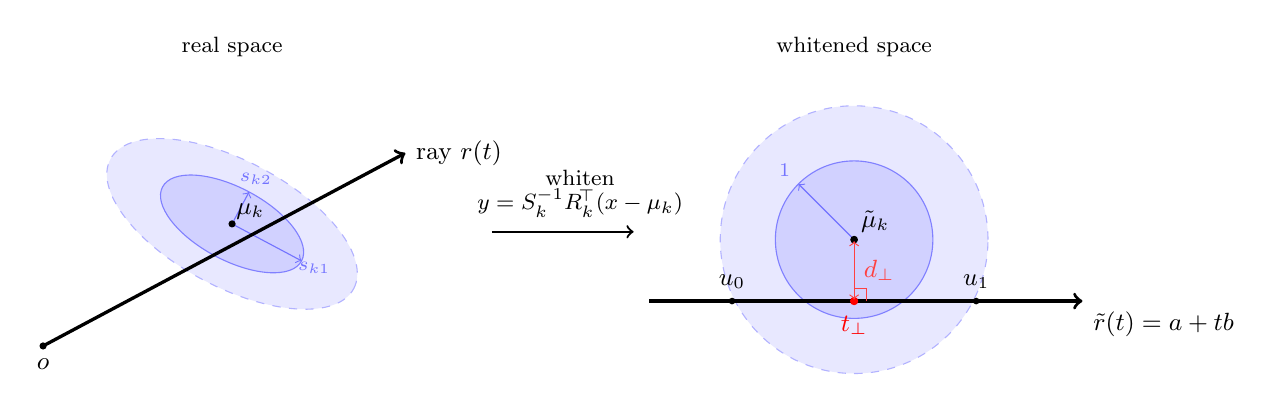
\begin{tikzpicture}[every node/.style={font=\small}]
    % ============ LEFT: real space (anisotropic, tilted) ============
    \node[font=\footnotesize] at (0.3,2.45) {real space};
    \begin{scope}[shift={(0.3,0.2)}, rotate=-28]
      \fill[blue!9]  (0,0) ellipse (1.75 and 0.8);
      \fill[blue!18] (0,0) ellipse (1.0 and 0.46);
      \draw[blue!50] (0,0) ellipse (1.0 and 0.46);
      \draw[blue!30,dashed] (0,0) ellipse (1.75 and 0.8);
      \draw[blue!55,->] (0,0) -- (1.0,0) node[pos=1.18,font=\scriptsize] {$s_{k1}$};
      \draw[blue!55,->] (0,0) -- (0,0.46) node[pos=1.4,font=\scriptsize] {$s_{k2}$};
    \end{scope}
    \fill (0.3,0.2) circle (1.3pt) node[above right=-2pt] {$\bm{\mu}_k$};
    \draw[->,very thick] (-2.1,-1.35) -- (2.5,1.1) node[right] {ray $\bm{r}(t)$};
    \fill (-2.1,-1.35) circle (1.3pt) node[below=1pt] {$\bm{o}$};
    % ============ whitening arrow ============
    \draw[->,thick] (3.6,0.1) -- (5.4,0.1);
    \node[align=center,font=\footnotesize] at (4.72,0.58)
      {whiten\\[-1pt] $\bm{y}=S_k^{-1}R_k^{\!\top}(\bm{x}-\bm{\mu}_k)$};
    % ============ RIGHT: whitened space (isotropic) ============
    \begin{scope}[shift={(8.2,0)}]
      \node[font=\footnotesize] at (0,2.45) {whitened space};
      \fill[blue!9]  (0,0) circle (1.7);
      \fill[blue!18] (0,0) circle (1.0);
      \draw[blue!50] (0,0) circle (1.0);
      \draw[blue!30,dashed] (0,0) circle (1.7);
      \draw[blue!55,->] (0,0) -- (-0.707,0.707) node[pos=1.25,font=\scriptsize] {$1$};
      \fill (0,0) circle (1.4pt) node[above right=-1pt] {$\tilde{\bm{\mu}}_k$};
      \def\yray{-0.78}
      \draw[->,very thick] (-2.6,\yray) -- (2.9,\yray) node[below right] {$\tilde{\bm{r}}(t)=\bm{a}+t\bm{b}$};
      \fill[red] (0,\yray) circle (1.5pt);
      \node[red,below=2pt] at (0,\yray) {$t_\perp$};
      \draw[<->,red!75] (0,-0.02) -- (0,\yray+0.02) node[midway,right] {$d_\perp$};
      \draw[red!75,thin] (0.16,\yray) -- (0.16,\yray+0.16) -- (0,\yray+0.16);
      \fill (-1.55,\yray) circle (1.2pt) node[above=1pt] {$u_0$};
      \fill ( 1.55,\yray) circle (1.2pt) node[above=1pt] {$u_1$};
    \end{scope}
  \end{tikzpicture}%
  }
  \caption{Analytic optical depth via whitening. \emph{Left:} in real space primitive $k$ is an
  anisotropic Gaussian (rotation $R_k$, per-axis scales $s_{ki}$, centre $\bm{\mu}_k$) and the ray
$\bm{r}(t)$ cuts it at an angle. \emph{Right:} whitening
  $\bm{y}=S_k^{-1}R_k^{\!\top}(\bm{x}-\bm{\mu}_k)$ maps the primitive to a unit-isotropic Gaussian at
  the origin (unit radius marked) and the ray to $\tilde{\bm{r}}(t)=\bm{a}+t\bm{b}$; the density now
depends only on distance from the origin,
  so completing the square splits it into a constant peak set by the perpendicular distance $d_\perp$
  (closest approach $t_\perp$, whitened speed $w=\lVert\bm{b}\rVert$) and a one-dimensional Gaussian
  along the ray. The optical depth between whitened endpoints $u_0,u_1$ is then
  $C_k'\,[\operatorname{erf}(u_1)-\operatorname{erf}(u_0)]$, monotonic in the endpoint and hence
  invertible by a single $\operatorname{erf}^{-1}$ (\Cref{sec:analytic-od}).}
  \label{fig:optical-depth}
\end{figure}

\section{Sort-free scatter sampling}
\label{sec:adt}

A volumetric path tracer must sample the distance to the next collision in proportion to the collision
density $\sigma_t(\bm{r}(t))\,T(t)$, i.e.\ draw a free flight (\Cref{sec:volumetric-light-transport}).
For a single homogeneous medium this means solving $\tau(t) = -\ln(1-\xi)$ for an exponentially
distributed target; for the \emph{sum} of overlapping primitives the reference does it by marching and
root-finding. This renderer avoids both by appealing to the structure of decomposition
tracking~\cite{Kutz2017}.

\paragraph{The argmin rule.} Decomposition tracking rests on the fact that a free flight through a sum
of components is distributed as the \emph{minimum} of independent free flights through each component
taken separately. Each primitive here \emph{is} such a component and, by \Cref{sec:analytic-od}, can
draw its own free flight in closed form. It samples a per-primitive target
$\tau_k = -\ln(1-\xi_k)$ with $\xi_k\sim\mathcal{U}[0,1)$, then inverts to the distance $t_k$ at which
primitive $k$ alone reaches $\tau_k$. The scattering event is the nearest of these,
\[
  t_{\text{scatter}} = \min_k t_k ,
\]
taken in a single linear pass over the ray's primitives (those in the active set, plus those in the
hit buffer). The reference marches the ray and root-finds the scatter distance within each segment,
selecting the next boundary by a running minimum at every step. This scheme needs neither
march nor root-find: the per-primitive inverse is exact (one $\operatorname{erf}^{-1}$), so a single
argmin over closed-form free flights gives the scatter point directly. The minimum reproduces
\emph{exactly} the distribution the reference's marching produces (it is the decomposition-tracking
identity, not an approximation), and the scatter \emph{distance} $t^\star$ is the result of this single
pass (\Cref{alg:argmin}).

\paragraph{The hit buffer's life cycle.} One kept optimisation and one instructive negative
result (\Cref{ch:optimization}) both turn on the buffer's life cycle, which is therefore described in full here.
During the single trace, the any-hit program only \emph{appends} ``primitive
$k$, entered at $t_{\text{entry}}$'' to the per-ray hit buffer (\Cref{sec:collection}). When
traversal ends, the renderer holds the ray's complete set of primitives, and reads it exactly
twice. The \emph{first} read is the argmin above: one draw per primitive, keep the nearest. The
\emph{second} read rebuilds, at the winning distance $t^\star$, the set of primitives whose spans
contain it---the scatter vertex's active set---with no new trace. That set mixes the local albedo
($\sigma_t$-weighted over the containing primitives), evaluates shadow-ray transmittance from
inside the overlap, and seeds the next bounce's containment. The buffer's fixed compile-time capacity
is the cap of \Cref{sec:gpu-impl}, sized per asset; the attempt to delete the buffer altogether is
the negative result of \Cref{sec:autopsies}.

\paragraph{Why the minimum is exact.} The identity is a one-line consequence of independence. Each $t_k$
is drawn from primitive $k$'s own free-flight law, so $\Pr[t_k > t] = e^{-\tau_k(t)}$---its
transmittance. The per-primitive draws use independent uniforms $\xi_k$, hence
\[
\begin{aligned}
  \Pr\!\big[\min_k t_k > t\big]
  &= \prod_k \Pr[t_k > t] = \prod_k e^{-\tau_k(t)} \\
  &= \exp\!\Big(-\!\sum_k \tau_k(t)\Big) = e^{-\tau(t)} = T(t),
\end{aligned}
\]
the transmittance of the \emph{combined} medium $\sigma_t=\sum_k\sigma_{t,k}$ (optical depth is additive
over overlapping primitives). So $t_{\text{scatter}}=\min_k t_k$ has exactly the combined free-flight
distribution with c.d.f.\ $1-T(t)$: the argmin is an exact sample from the mixture, not an
approximation. Exactness holds for the $3\sigma$-bounded kernel both renderers use.
\Cref{ch:validation} reports a small convergence-stable residual at heavy overlap whose cause is
not yet isolated; a double-precision $\operatorname{erf}^{-1}$ test rules out finite precision. The
candidate causes are next-event shadow transmittance evaluated from inside overlapping primitives,
active-set bookkeeping, and a since-found reference-side issue (\Cref{ch:conclusion}). Unlike the
delta/null-tracking that decomposition tracking normally requires, no majorant (the
bounding density delta tracking homogenises against, \Cref{sec:volumetric-mc})
and no null-scattering events appear here, because every per-primitive free flight is itself drawn in
closed form (\Cref{sec:analytic-od}). The analytic invertibility is what removes the stochastic
tracking entirely.

\begin{algorithm}[htp]
\caption{Argmin scatter sampling for one ray (one path bounce).}
\label{alg:argmin}
\begin{algorithmic}[1]
\Require ray $\bm{r}$; active set $A$ (primitives containing the origin); hit buffer $H$ of entries
$(t_{\text{entry}}, k)$ from one trace; per-primitive analytic exit $t_{\text{exit}}(k)$ (\Cref{sec:collection})
\Ensure scatter distance $t^\star$, or \textsc{Escape}
\State $t^\star \gets +\infty$
\Function{Try}{$k$, $t_{\text{start}}$} \Comment{free flight of primitive $k$, measured from $t_{\text{start}}$}
  \State $\tau \gets -\ln(1-\xi)$, \quad $\xi \sim \mathcal{U}[0,1)$ \Comment{drawn independently each call}
  \State $t \gets \textproc{inv\_cdf\_span}(\bm{r}, t_{\text{start}}, \tau)$ \Comment{span-restricted inverse from $t_{\text{start}}$}
  \If{$t_{\text{start}} \le t \le t_{\text{exit}}(k)$ \textbf{ and } $t < t^\star$}
    \State $t^\star \gets t$ \Comment{nearest collision so far (the argmin)}
  \EndIf
\EndFunction
\ForAll{$k \in A$}
  \State \Call{Try}{$k$, $0$} \Comment{origin inside: start at $0$}
\EndFor
\ForAll{$(t_{\text{entry}}, k) \in H$}
  \State \Call{Try}{$k$, $t_{\text{entry}}$} \Comment{entered mid-ray: start at the entry}
\EndFor
\If{$t^\star = +\infty$} \State \Return \textsc{Escape} \EndIf
\State \Return $t^\star$
\end{algorithmic}
\end{algorithm}

\paragraph{Avoiding a rejection bias.} Both candidate categories use the same span-restricted inverse
\textproc{inv\_cdf\_span}$(\bm{r}, t_{\text{start}}, \tau)$, which solves $\tau_k(t_{\text{start}}, t) =
\tau$ directly for the distance $t$. A primitive the ray is already inside starts at $t_{\text{start}}=0$;
a primitive entered mid-ray starts at its \emph{entry} distance, $t_{\text{start}}=t_{\text{entry}}$. The
alternative would use the unrestricted full-Gaussian inverse and reject samples that land before the
entry. That would bias the result, because the rejected probability mass is dropped rather than
re-rolled.
Shifting the error-function reference to $t_{\text{start}}$ instead keeps every candidate unbiased by
construction. (The implementation specialises $t_{\text{start}}=0$ to a separate \textproc{inv\_cdf}, a
minor optimisation.)

\paragraph{Novelty and prior art.} The components of this scheme are individually known: the
minimum-of-free-flights identity is decomposition tracking~\cite{Kutz2017}; the closed-form Gaussian
optical depth is from the reference~\cite{DSYG}; and the sort-free \emph{spirit} mirrors stochastic
splatting~\cite{StochasticSplats2025} on the rasterisation side. What is new here is the
combination: applying analog decomposition tracking to ray-traced Gaussian kernel-mixture volumes.
The analytic per-primitive inverse makes each component's free flight a closed-form draw, and
the argmin replaces the reference's marching and root-finding entirely. The approach was suggested by
Condor, the lead author of the reference~\cite{DSYG} (personal communication, 2026), and is realised and
validated here, to the author's knowledge for the first time for this representation.

\paragraph{Complexity.} Per scattering bounce the work is $O(N + A + H)$. An $O(N)$ scan maintains the
active set against the scene's $N$ primitives; an $O(A + H)$ pass over the $A$ active and $H$
newly entered primitives takes the argmin. This replaces the reference's per-bounce boundary
marching (an $O(H^2)$ running-minimum selection across segments) and its per-segment root-find with
closed-form work. Because the argmin needs no ordering, ordered boundary processing disappears
from the common (scattering) path altogether. The $O(N)$ active-set
scan is the dominant per-bounce cost of the \emph{base} algorithm. \Cref{ch:optimization} runs the full
scan only at the first bounce and inherits the active set thereafter, so the optimised renderer is no
longer $O(N)$ per bounce.

\section{Direct lighting and the path-tracing loop}
\label{sec:direct-lighting}

At each scattering vertex the renderer estimates direct illumination from the environment map by
next-event estimation under multiple importance sampling (\Cref{sec:volumetric-light-transport}).
The environment map is an image-based model of distant illumination surrounding the scene, sampled
as an infinitely far emitter. Two sampling strategies run per vertex, each tracing one
shadow ray: the first draws its direction from the environment map's luminance distribution (luminance: the
standard scalar brightness of an RGB value, a fixed weighted sum of the three channels), the second from the Henyey--Greenstein phase function. Each strategy is
weighted by the balance heuristic, with transmittance along its shadow ray from the
analytic optical depth of \Cref{sec:analytic-od}. Indirect light is carried by the phase-sampled continuation ray, whose direct
environment contribution is suppressed so it is not double-counted against next-event estimation.
\Cref{ch:optimization} replaces this two-shadow-ray estimator with an optional
resampled-importance-sampling variant that traces a single shadow ray, keeping the MIS scaffold intact.

The primary (camera) ray's direct contribution is treated specially. Rather than relying on the path to
escape the medium and hit the environment, the renderer adds the analytic camera-to-environment term
$T_{\text{cam}}\,L_{\text{env}}$ at bounce zero. Here $T_{\text{cam}}$ is the closed-form transmittance
through the medium along the view ray. This \emph{Rao--Blackwellises} the otherwise high-variance
escape contribution. By the Rao--Blackwell theorem~\cite{Rao1945,Blackwell1947}, replacing a random
estimator by its analytic conditional expectation ($T_{\text{cam}}\,L_{\text{env}}$) can only lower
variance. The random estimator here is whether a stochastically-sampled path happens to escape the
medium and reach the environment; the replacement costs just one extra transmittance ray. Paths are terminated by Russian roulette beyond a configurable depth,
with survival probability set to the largest colour channel of the path's
\emph{throughput}---the running product of per-event weights, i.e.\ the fraction of its
original radiance the path still carries---clamped to \num{0.99}; surviving throughput
is reweighted to keep the estimator unbiased.

Samples are accumulated by Welford's single-pass online mean~\cite{Welford1962} (and variance, when adaptive sampling is
enabled). Arbitrarily many samples per pixel can thus be folded in across launches, without storing
per-sample data and without catastrophic cancellation. Sample batches are processed within a single
kernel launch, amortising launch overhead and keeping the accumulator in registers across the batch.

\section{Data structures and GPU configuration}
\label{sec:gpu-impl}

\paragraph{Acceleration structure.} The scene is built as a two-level OptiX structure. A single
geometry acceleration structure (GAS) holds one \emph{unit sphere}, built from OptiX's~\cite{Optix} built-in sphere
primitive (\texttt{OPTIX\_BUILD\_INPUT\_TYPE\_SPHERES}) so that ray--sphere intersection uses the
vendor-optimised built-in intersector rather than a custom program. (The built-in sphere is exact but,
unlike triangle intersection, does not execute on the dedicated ray-tracing cores;
\Cref{sec:icosphere} measures this choice against the reference's tessellated icospheres.) Each Gaussian primitive is then an \emph{instance} of that
GAS in an instance acceleration structure (IAS). The instance carries the affine transform that maps
the unit sphere to the primitive's centre, anisotropic scale, and orientation (from its rotation
quaternion). Thousands of distinct ellipsoids thus share a single sphere GAS, and the per-primitive
geometry lives entirely in the instance transforms. Both structures are built with
\texttt{OPTIX\_BUILD\_FLAG\_PREFER\_FAST\_TRACE}: favouring traversal speed over build time is the
right trade for a renderer that builds once and traces for many samples. They also set
\texttt{OPTIX\_BUILD\_FLAG\_ALLOW\_COMPACTION}, standard practice that shrinks the built
structure at no traversal cost.

\paragraph{Per-ray state.} Two per-ray containers dominate the kernel's footprint. The hit buffer
(\Cref{sec:collection}) is a fixed-capacity \texttt{HitBufferSoA}. The active set is a small membership
structure whose representation is chosen at compile time by scene size. For up to \num{256} primitives a
\emph{bit vector} gives $O(1)$ insert, erase, and test in $N/8$ bytes. Beyond that a compact unsorted
array gives $O(k)$ operations, in space proportional to the maximum overlap rather
than the scene size. The relevant capacities (the active-set bound and the hit-buffer length) are
compile-time constants and should be as small as safety allows. The two differ, though, in how much
tightness matters. Both costs flow from one fact: the per-ray hit buffer and active set live in thread-local memory,
which the driver reserves for the device's maximum resident thread count. An oversized cap therefore both
lowers occupancy and sets a scene-independent floor on device memory. A universal ``safe'' build
($512/512$, the cap a user without tooling would pick) was measured against the per-asset-tuned
builds, interleaved at locked clocks. It cost
$+14\,\%$ frame time on the cloud, $+8\,\%$ on the explosion, and
$+7\,\%$ on the bunny,\footnote{The bunny figure used the \num{80}/\num{496} build; the shipped bunny cap is \num{80}/\num{528} (\Cref{tab:vram}), but the penalty is dominated by the active-set
inflation ($80\to512$ below) and is insensitive to the hit cap at this level.} and was within
run-to-run jitter on the tornado. The cost is not extra
computation but reduced occupancy: a larger per-ray reservation lets fewer rays run on the GPU at once,
so it hides less of the memory-access latency that dominates this kernel (\Cref{sec:bottleneck}). The
effect is asset-dependent and does not reduce to any single cap.

The safe build reserves a flat $1200\,$MiB on every asset,
whereas the per-asset-tuned builds use $578$--$900\,$MiB---a saving of $0.30$--$0.62\,$GiB
($25$--$52\,\%$). The effect is large enough to flip the cross-renderer memory comparison. Tuned, the
renderer's peak device memory on the cloud ($578\,$MiB) sits \emph{below} the Mitsuba reference's
($838\,$MiB) on the same scene; the untuned safe build ($1200\,$MiB) exceeds it. The active set
(\num{2} bytes per entry) tolerates \emph{modest} headroom: doubling its
capacity beyond the cloud's worst case measured as timing-neutral in an interleaved A/B (differences
under the run-to-run jitter), with renders numerically equivalent. What ultimately matters is the total
reserved bytes per ray, not which cap. The hit buffer consumes them three times faster per entry and is
the more sensitive cap; a large active-set increase ($80\to512$ on the bunny) is not free either.

The caps are sized from measured demand. A \texttt{--measure-caps} render mode counts the
true per-ray hit demand and per-vertex overlap of the actual workload.\footnote{Its counters are
cap-independent: the collection shader counts \emph{dropped} hits too, and point-overlap is an
exhaustive containment scan rather than the clipped active set.} A one-command calibration wrapper
measures the asset's binding stress on two seeds, writes the margined constants, rebuilds, and
verifies zero overflow on a deliberately \emph{unmeasured} seed. For the primary cloud scene the
measured worst case is \num{45} simultaneously overlapping primitives and \num{85} entries on the
worst ray. This sits comfortably inside
the calibrated capacities, and the runtime counter below records zero overflows. A complementary
offline estimator Monte~Carlo-samples points and lines through the scene's bounding box against each
primitive's $3\sigma$ ellipsoid, giving a cheap camera-independent \emph{estimate} before any build
(\Cref{tab:overlap}). It is an estimate, not a guaranteed bound. Measurement on the \num{25600}-Gaussian
bunny shows why the in-render counters, not the estimator, are the sizing authority. The whole-bbox
bound over-sized the bunny's active set four-fold: a margined cap of \num{320} from the \num{245}
predicted overlap of \Cref{tab:overlap}, vs.\ \num{71} measured. Its sampled lines \emph{under}-shot the
worst observed ray by ${\sim}20\,\%$ (\num{387} vs.\ \num{464}), surviving only on its safety margin.
A deliberately degenerate collinear stress test
exercises the overflow path (\Cref{ch:validation}). Because no static cap can be guaranteed sufficient
on every scene, a device-side overflow counter flags at runtime any ray that exceeds a capacity, so
excess overlap is flagged rather than silently corrupting the image.

\paragraph{Megakernel rationale.} The entire bounce loop executes inside the ray-generation program: a
single \emph{megakernel}. The standard alternative is \emph{wavefront} path tracing~\cite{Laine2013},
in which each stage of the path---ray traversal, scattering, shading---is a separate kernel launch.
Per-ray state is carried between stages through global memory, with stream compaction
(repacking the still-alive rays into a dense array, so adjacent threads keep doing
identical work) between stages to
keep GPU warps coherent. Keeping the whole loop in one kernel fits this workload. The per-bounce arithmetic is light (a few
error functions and a phase evaluation), but the per-ray \emph{state} that must persist across
bounces---mainly the active set---is comparatively large. A wavefront would have to stream that state
to and from global memory every bounce; the megakernel keeps it in registers and per-thread local memory
(L1/L2-resident), paying no global round-trips. \Cref{ch:optimization} reports the experiment that confirms this: a wavefront
refactor, though correct, was dramatically slower. Moving the persistent per-ray state to
global memory is fatal for an algorithm whose per-bounce compute is otherwise so cheap.

\paragraph{Implementation.}{\sloppy Beyond OptiX and a few small header-only utilities (PLY and EXR (HDR image) I/O,
logging, and command-line parsing), the renderer has no external dependencies---in particular no
rendering framework---which keeps the codebase compact and straightforward to extend. Optional features are toggleable without touching the core renderer. The OptiX denoiser
and volumetric product-RIS are \emph{runtime} flags (\texttt{--denoise};
\texttt{--ris}, with candidate count \texttt{--ris-candidates}). Adaptive sampling and a fast \texttt{erf} (a polynomial approximation to $\operatorname{erf}$,
numerically validated within the gates of \Cref{ch:validation}) are compile-time
switches. The rendering parameters themselves are likewise exposed on the command line, so an experiment is
specified entirely by its invocation. Sampling is set by samples per pixel (\texttt{--spp}) and RNG seed
(\texttt{--seed}); the medium by the density scale (\texttt{--sigma-multiplier}) and phase anisotropy
(\texttt{--phase-g}). Path termination is set by the maximum path depth and Russian-roulette schedule
(\texttt{--max-depth}, \texttt{--rr-depth}, \texttt{--rr-max-survival}). The remaining controls are the optional firefly clamp (\texttt{--firefly-clamp}) and
pixel filter (\texttt{--filter-width}), plus the cap-measurement mode
(\texttt{--measure-caps}) behind the calibration above.\par}

\paragraph{Implementation philosophy and availability.} The codebase was written to outlive this
thesis. The host side is compact, modern object-oriented C++. Resource management is uniformly
RAII: no manual allocation, and CUDA and OptiX handles live in owning wrapper types. Errors propagate
through explicit result types rather than silent fallbacks, and ownership and memory-layout
decisions are documented at the point where they are made. Experimental features are isolated
behind compile-time guards that leave the production binary byte-identical when disabled.
Because a disabled feature leaves the binary untouched, an A/B such as the icosphere
comparison (\Cref{sec:icosphere}) measures only the change under test. Rendering parameters are runtime flags, so every experiment in this thesis is
fully specified by a single documented invocation. The campaign scripts that produced each
result figure are kept alongside the sources. The renderer, its test scenes, and those scripts are
available as open source.\footnote{\url{https://github.com/kfernandez31/cuda-volprim}}
